% Copyright 2026 Sreeram Anil
% SPDX-License-Identifier: CC-BY-4.0
% =============================================================================
%  Extended information filter — classical Kalman family
% =============================================================================
\chapter{Extended Information Filter (EIF)}
\label{ch:eif}

\section*{At a glance}
\begin{tabular}{@{}l>{\raggedright\arraybackslash}p{0.76\textwidth}@{}}
Family & classical Kalman (information form) \\
Header & \texttt{include/estkit/filters/eif.hpp} \\
Registered name & \texttt{EIF} \\
State dimension & $n_x = 4$ (cell model) --- generic in $n_x, n_u, n_y$ \\
Propagated quantities & $\bm{Y} = \mP\inv$, $\bm{\upsilon} = \bm{Y}\xhat$ \\
Cost per step & $\mathcal{O}(n_x^3)$, three $n_x\times n_x$ inversions; $1.17$--$1.24\,\SI{}{\micro\second}$/step \\
Primary references & \cite{mutambara1998,andersonmoore1979,maybeck1979,thrun2005} \\
\end{tabular}

\section{Motivation and aerospace/BMS relevance}
The information filter is the same estimator as the Kalman filter written in terms of the
inverse covariance. This exchanges the difficulty of the two halves of the cycle: the
measurement update becomes a \emph{sum} and the time update becomes the hard part. Three
consequences make the trade worthwhile in specific architectures.

First, additivity. $N$ conditionally independent sensors contribute $N$ terms
$\mH_i^\T\mR_i\inv\mH_i$ that can be computed on separate processors, transmitted, and summed
in any order with no synchronisation. This is the mathematical basis of decentralised and
federated filters~\cite{mutambara1998,carlson1990federated} and is directly relevant to a
battery pack, where dozens of cell-monitoring ASICs each produce a voltage measurement that
must be fused by one master.

Second, ignorance is representable. ``No prior information'' is $\bm{Y} = \bm{0}$ exactly, whereas
a covariance filter must fake it with a large $\mP_0$ and then suffer the numerical
consequences. A BMS that wakes up after a long rest with no stored SOC can start the EIF from
$\bm{Y}=\bm0$ and let the first OCV measurement define the estimate.

Third, sparsity. In large problems (SLAM, pack-level estimation with weak inter-cell
coupling) $\bm{Y}$ is nearly sparse while $\mP$ is dense, which is the basis of the sparse
extended information filter~\cite{thrun2005}. None of these advantages is exercised by a
single-cell, single-sensor benchmark; this chapter therefore serves to \emph{validate} the
information form against the EKF and to quantify what the change of variables costs.

\section{Problem statement and assumptions}
Model \eqref{eq:ekf-proc}--\eqref{eq:ekf-meas}. Define
\begin{equation}
\bm{Y}_k = \mP_k\inv \in\real^{n_x\times n_x} \quad\text{(information matrix)},\qquad
\bm{\upsilon}_k = \bm{Y}_k\xhat_k \in\real^{n_x} \quad\text{(information vector)}.
\label{eq:eif-defs}
\end{equation}
The information form requires $\mP$ to be invertible at all times, hence $\mQ\succ0$; the
time update derived below additionally requires $\mF$ to be invertible, which holds for any
discretisation of a physical system (and here $\mF=\diag(1,a_1,a_2,a_h)$ with all entries in
$(0,1]$).

\section{Derivation}
\paragraph{Measurement update.} Starting from the covariance-form Joseph update and applying
the matrix inversion lemma, or directly from the Gaussian log-density
\begin{equation}
-2\log p(\vx\mid\vy_{1:k}) = (\vx-\xminus_k)^\T(\Pminus_k)\inv(\vx-\xminus_k)
 + (\vy_k-h(\vx,\vu_k))^\T\mR\inv(\vy_k-h(\vx,\vu_k)) + \text{const},
\label{eq:eif-logpost}
\end{equation}
linearising $h$ about $\xminus_k$ and collecting the quadratic and linear terms in $\vx$:
\begin{align}
\bm{Y}^+_k &= \bm{Y}^-_k + \mH_k^\T\mR\inv\mH_k, \label{eq:eif-mu-Y}\\
\bm\upsilon^+_k &= \bm\upsilon^-_k + \mH_k^\T\mR\inv\left[\vy_k - h(\xminus_k,\vu_k) + \mH_k\xminus_k\right].
\label{eq:eif-mu-y}
\end{align}
The bracket is the linearised measurement ``referred back to the origin''; for a linear model
it is simply $\vy_k$. Equations \eqref{eq:eif-mu-Y}--\eqref{eq:eif-mu-y} contain no inverse of
an $n_x\times n_x$ matrix and no gain: the update is an addition of the information supplied
by the sensor, which is why it parallelises trivially.

\paragraph{Time update.} This is where the work moves. In covariance form
$\Pminus_k = \mF\Pplus_{k-1}\mF^\T+\mQ$, so
\begin{equation}
\bm{Y}^-_k = \left[\mF(\bm{Y}^+_{k-1})\inv\mF^\T + \mQ\right]\inv .
\label{eq:eif-tu-naive}
\end{equation}
Define $\bm{M} = \mF^{-\T}\bm{Y}^+_{k-1}\mF\inv$, so that
$\mF(\bm{Y}^+_{k-1})\inv\mF^\T = \bm{M}\inv$. The Woodbury identity
$(\bm{M}\inv+\mQ)\inv = \bm{M} - \bm{M}(\bm{M}+\mQ\inv)\inv\bm{M}$ then gives the standard information-form
time update~\cite[\S6.3]{andersonmoore1979}
\begin{equation}
\boxed{\;\bm{Y}^-_k = \bm{M} - \bm{M}\left(\bm{M} + \mQ\inv\right)\inv\bm{M}, \qquad
 \bm{M} = \mF^{-\T}\bm{Y}^+_{k-1}\mF\inv .\;}
\label{eq:eif-tu}
\end{equation}
For the nonlinear mean the propagation is unchanged, $\xminus_k = f(\xplus_{k-1},\vu_{k-1})$,
and $\bm\upsilon^-_k = \bm{Y}^-_k\xminus_k$. Note the structural asymmetry: the measurement
update needs $\mR\inv$ ($n_y\times n_y$, here a scalar) while the time update needs $\mF\inv$,
$\mQ\inv$ and one $n_x\times n_x$ solve.

\paragraph{Recovering the estimate.} $\xhat_k = \bm{Y}_k\inv\bm\upsilon_k$ and $\mP_k=\bm{Y}_k\inv$.
Because the benchmark adapter needs $\soc$ and $\sigma_\soc$ at every sample, and because the
nonlinear $f$ and $h$ must be evaluated at $\xhat$, the implementation recovers them through a
cached, lazily evaluated inversion: a \code{dirty} flag is set by \code{predict} and
\code{update} and cleared by the first accessor that needs $(\xhat,\mP)$.

\begin{proposition}\label{prop:eif-equiv}
For the same linearisation points, \eqref{eq:eif-mu-Y}--\eqref{eq:eif-tu} produce the same
estimate and covariance as the EKF of Chapter~\ref{ch:ekf}.
\end{proposition}
This is an algebraic identity, and it is verified numerically below; the value of the chapter
is that the identity holds in \emph{practice}, i.e. that the extra inversions do not destroy
it.

\section{Algorithm}
\begin{algorithm}[H]
\caption{EIF --- one sampling period}
\begin{algorithmic}[1]
\Require $\bm{Y}^+_{k-1},\bm\upsilon^+_{k-1},\vu_{k-1},\vy_k,\vu_k$
\State recover $\xplus_{k-1}\gets(\bm{Y}^+_{k-1})\inv\bm\upsilon^+_{k-1}$ if not cached
\State \textbf{Time update:} $\mF\gets\partial f/\partial\vx|_{\xplus_{k-1},\vu_{k-1}}$;\;
       $\xminus_k\gets f(\xplus_{k-1},\vu_{k-1})$
\State $\bm{M}\gets\mF^{-\T}\bm{Y}^+_{k-1}\mF\inv$;\;
       $\bm{Y}^-_k\gets\bm{M}-\bm{M}(\bm{M}+\mQ\inv)\inv\bm{M}$;\;
       $\bm\upsilon^-_k\gets\bm{Y}^-_k\xminus_k$
\State \textbf{(fall-back)} if $\mF$ or $\mQ$ is singular: $\bm{Y}^-_k\gets(\mF\Pplus_{k-1}\mF^\T+\mQ)\inv$
\State \textbf{Predicted measurement:} $\yhat_k\gets h(\xminus_k,\vu_k)$
\State \textbf{Measurement update:} $\mH\gets\partial h/\partial\vx|_{\xminus_k,\vu_k}$
\State $\bm{Y}^+_k\gets\bm{Y}^-_k+\mH^\T\mR\inv\mH$;\;
       $\bm\upsilon^+_k\gets\bm\upsilon^-_k+\mH^\T\mR\inv(\vy_k-\yhat_k+\mH\xminus_k)$
\State $\Pplus_k\gets(\bm{Y}^+_k)\inv$;\; $\xplus_k\gets\Pplus_k\bm\upsilon^+_k$
\State \textbf{if} constraints enabled \textbf{then} $\xplus_k\gets\Pi(\xplus_k)$, $\bm\upsilon^+_k\gets\bm{Y}^+_k\xplus_k$
\Ensure $\bm{Y}^+_k,\bm\upsilon^+_k$ (and the cached $\xplus_k,\Pplus_k$)
\end{algorithmic}
\end{algorithm}

\section{Application to the battery model}
Because $\mF=\diag(1,a_1(T),a_2(T),a_h(i))$ the inverse $\mF\inv$ is a diagonal reciprocal and
$\bm{M} = \mF^{-\T}\bm{Y}\mF\inv$ costs $n_x^2$ divisions instead of two matrix products --- a
diagonal $\mF$ is the best case for the information form. $\mQ$, in contrast, is
\emph{not} diagonal: it is $\bm b\bm b^\T\sigma_i^2 + \diag(q_{\text{floor}}^2)$, a rank-one
current-noise term plus a floor, so $\mQ\inv$ is a genuine $4\times4$ inverse. (A
Sherman--Morrison update on the rank-one part would reduce this to $\mathcal{O}(n_x^2)$; it is
not implemented because the generic model interface only exposes $\mQ$ itself.)

With $n_y=1$ the measurement update is $\mH^\T\mH/R$ --- a rank-one addition, four multiplies
--- which is a good illustration of the information form's asymmetry: what a covariance filter
does with an inverse and a gain, the information filter does with an outer product.

Options: \code{information\_time\_update = true} (use \eqref{eq:eif-tu}; setting it to
\code{false} selects the covariance-form fall-back and gives identical results),
\code{apply\_constraints = true}, \code{q\_scale = r\_scale = 1}.

\section{Implementation notes}
Three $4\times4$ inversions per step ($\mF\inv$, $\mQ\inv$, $(\bm{Y}^+)\inv$) plus one SPD solve
explain the measured $1.17$--$1.24\,\SI{}{\micro\second}$ against the EKF's
$0.44$--$0.48\,\SI{}{\micro\second}$: on this problem the information form costs $2.6\times$ an
EKF step and buys nothing, because there is one sensor and $\bm{Y}$ is dense.
The break-even point is the number of independent measurement channels: the covariance form
costs $\mathcal{O}(n_y^3)$ in the update, the information form $\mathcal{O}(n_x^3)$ in the
prediction, so the information form wins once $n_y\gtrsim n_x$ --- which is exactly the
pack-level situation.

Robustness: $\bm{Y}_0 = \mP_0\inv$ is replaced by $10^6\mI$ if $\mP_0$ is singular;
\eqref{eq:eif-tu} is attempted first and silently falls back to
$(\mF\Pplus\mF^\T+\mQ)\inv$ if either $\mF$ or $\mQ$ is numerically singular; the cached
$(\xhat,\mP)$ are only updated when the inversion succeeds, so a failed inversion leaves the
last good estimate in place rather than producing NaN. After constraint projection the
information vector is recomputed as $\bm\upsilon = \bm{Y}\xhat$ to keep the pair consistent.
\code{sizeof(Eif<EcmModel>)} is 4472\,bytes.

\section{Benchmark results}
\input{tables/cell_EIF.tex}
\begin{figure}[H]\centering
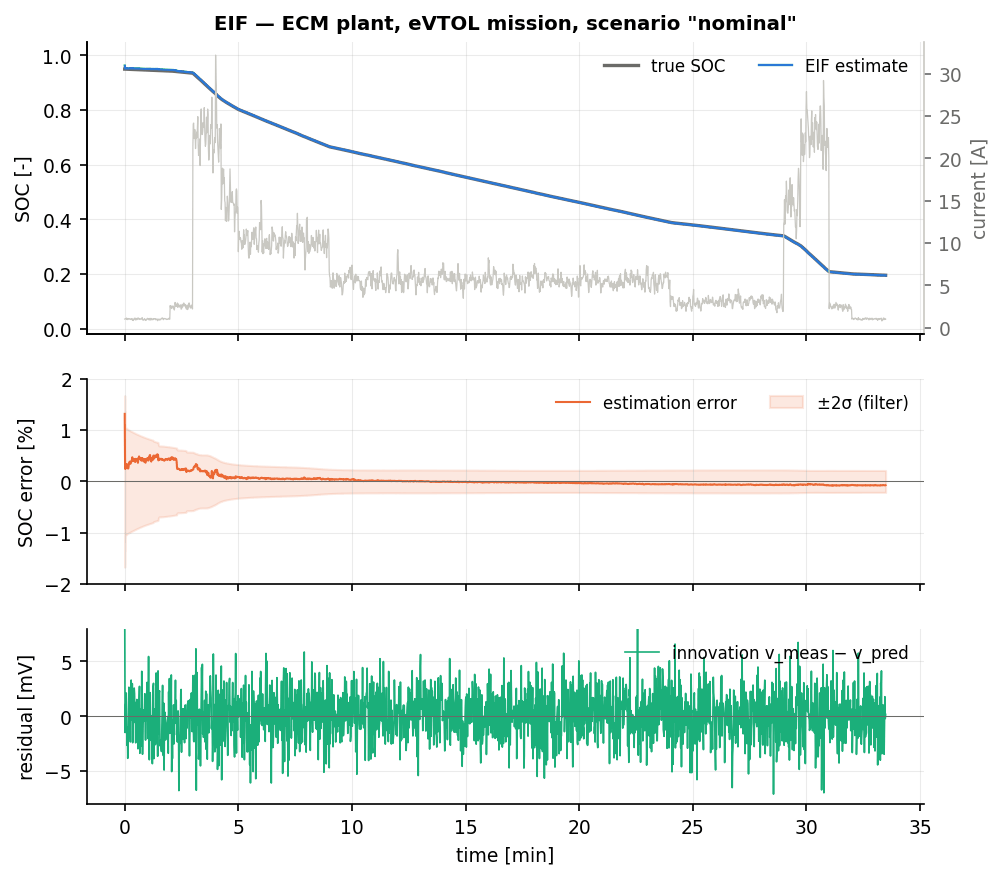
\includegraphics[width=\textwidth]{figures/cell_EIF_nominal.png}
\caption{EIF on the nominal eVTOL mission: true and estimated SOC (top), estimation error with the $\pm 2\sigma$ band when available (middle), voltage residual (bottom).}
\end{figure}
\begin{figure}[H]\centering
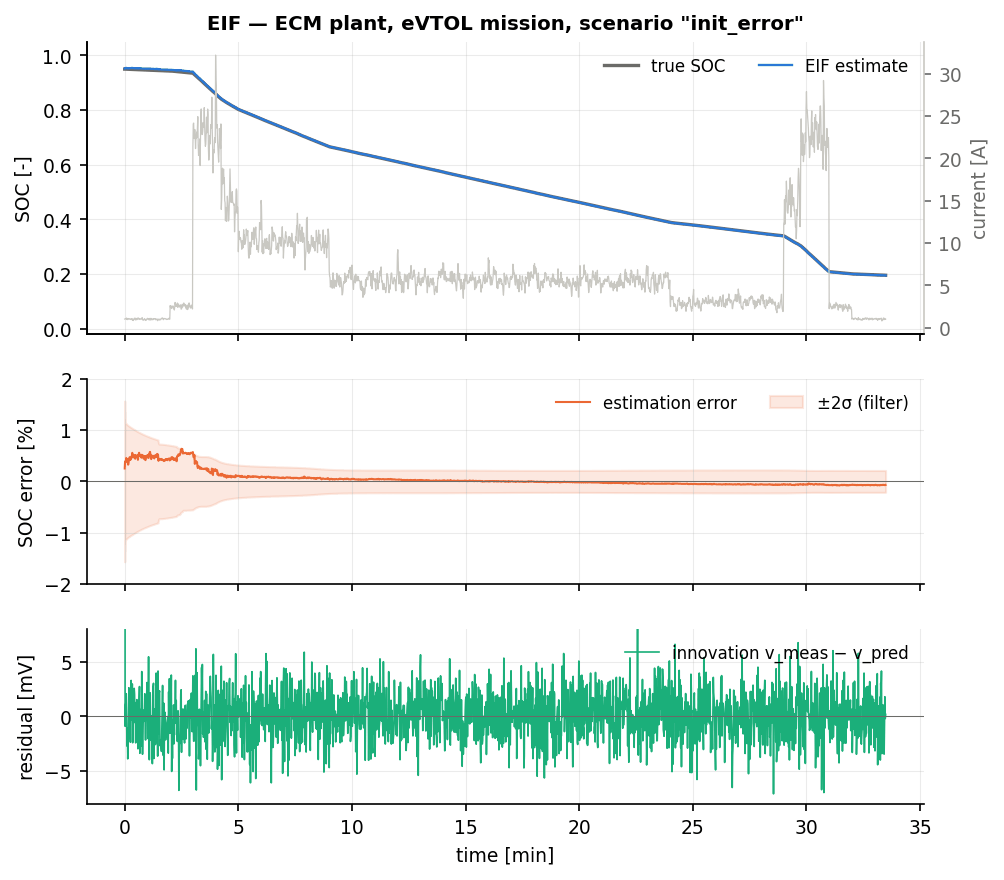
\includegraphics[width=\textwidth]{figures/cell_EIF_init_error.png}
\caption{EIF with a 35\,\% initial SOC error.}
\end{figure}

All numbers are three-seed means in per cent SOC.

The EIF reproduces the EKF exactly on every scenario of both plants, to all printed decimals:
ECM \texttt{nominal} $0.15/0.05\,\%$, \texttt{init\_error} $0.14/0.05\,\%$ with
$t_{\text{conv}} = 0$\,s, \texttt{current\_bias} $0.54/0.61\,\%$, \texttt{aged\_cell}
$1.18/1.52\,\%$, \texttt{param\_mismatch} $1.28/1.36\,\%$, \texttt{sensor\_dropout}
$0.72/0.46\,\%$, \texttt{preisach} $0.58/0.20\,\%$, \texttt{combined} $16.02/12.44\,\%$. A
direct element-wise comparison over a full nominal mission ($\num{18000}$ steps) gives
$\max\abs{\Delta\vx} = 1.9\times10^{-11}$ and $\max\abs{\Delta\mP} = 1.3\times10^{-14}$,
confirming Proposition~\ref{prop:eif-equiv} numerically. The discussion of
Chapter~\ref{ch:ekf} therefore applies without change, including the \texttt{combined} failure.

The $10^{-11}$ discrepancy is larger than the $10^{-14}$ of the square-root and U-D filters
(Chapters~\ref{ch:srekf}, \ref{ch:udekf}) --- a small but real indication that the information
form is the \emph{least} numerically favourable of the algebraically equivalent
implementations. That is expected: it squares the condition number twice over (once in
$\bm{Y} = \mP\inv$, once in $(\bm{M}+\mQ\inv)\inv$) where a square-root filter halves it. The
single-precision build shows the same tendency at the level of the estimates: on
\texttt{combined} the EIF gives $12.66\,\%$ in float against $11.90\,\%$ in double, the largest
float-double gap of the four EKF-equivalent implementations (EKF $12.21$, SR-EKF $12.21$,
UD-EKF $12.18\,\%$), while on \texttt{nominal} it is $0.03\,\%$ against $0.06\,\%$ --- noise, at
this level. At $n_x = 4$ the effect is still below the estimation error; at larger $n_x$ or with
near-deterministic states ($\mQ\to0$, where $\mQ\inv$ blows up) it would not be.

The cost, $1.17$--$1.24\,\SI{}{\micro\second}$ against the EKF's $0.44$--$0.48$ --- a factor of
$2.6$ --- is the price of the change of variables on a single-sensor problem. It is worth
restating that this is the worst case for the information form: with one measurement channel and
a dense $\mQ$, every structural advantage is absent.

\paragraph{SPM plant: structured model error.}
\begin{figure}[H]\centering
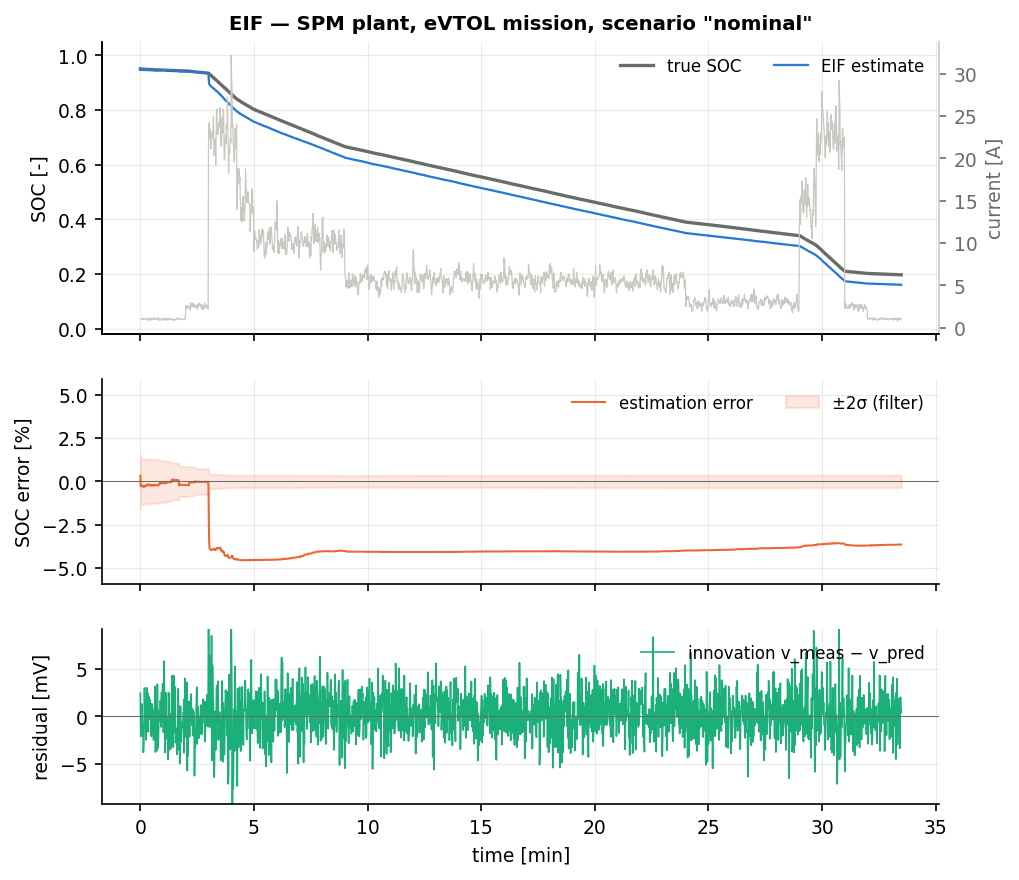
\includegraphics[width=\textwidth]{figures/cellspm_EIF_nominal.png}
\caption{EIF on the nominal mission with the electrochemical (SPM) plant; identical to the conventional EKF.}
\end{figure}
The SPM block of the table is a different kind of test. The plant is the electrochemical
single-particle model; the estimator still runs a 2-RC equivalent circuit, fitted to that plant,
which leaves a \emph{structured} residual of about $4$\,mV (Butler--Volmer kinetics and
solid-phase diffusion that no 2-RC circuit can reproduce) and a slow second branch,
$\tau_2 = 556$\,s. Over a $33$-minute mission a $556$\,s pole barely relaxes, so $v_2(t)$ is
close to an affine ramp --- and so is $\ocv(\soc(t))$ while the cell discharges at a roughly
constant rate. The two channels through which the measurement sees the state,
$(\partial\ocv/\partial\soc)\,\delta\soc$ and $-\delta v_2$, are therefore nearly collinear in
the information accumulated over the flight: the pair $(\soc, v_2)$ is close to unobservable,
and no filter can decide whether a persistent few-millivolt residual belongs to the slow RC
branch or to the state of charge. Because that direction is weakly observable, a $4$\,mV
structured error maps onto \emph{several per cent} of SOC instead of the
$4\,\text{mV}/0.8\,\text{V}\approx0.5\,\%$ a well-conditioned channel would give. This
$(\soc,v_2)$ ambiguity, not the size of the residual, is the mechanism behind the
$3.7$--$4.6\,\%$ band in which the whole classical family sits.

Being algebraically the EKF, the EIF inherits the EKF's SPM rows exactly: $3.65/3.73\,\%$ on
\texttt{nominal} with a voltage residual of only $1.02$\,mV, $7.35\,\%$ on \texttt{cold},
$5.69\,\%$ on \texttt{current\_bias}, $5.31\,\%$ on \texttt{sensor\_dropout}, $3.13\,\%$ on
\texttt{param\_mismatch}, $1.99\,\%$ on \texttt{outliers}. Nothing diverges;
$t_{\text{conv}} = 0$ on every SPM row, because the error is a bias rather than a drift.

The SPM rows are, however, the place where the information form's \emph{structural} argument
becomes concrete. The $(\soc,v_2)$ ambiguity is exactly a near-singular direction of
$\bm{Y}$: the information matrix accumulates almost nothing along it, and the filter's inability
to apportion the residual is visible as a small eigenvalue rather than as a large one in $\mP$.
An information filter makes that diagnosis directly --- monitor $\lambda_{\min}(\bm{Y})$ and
its eigenvector --- and it is also the natural place to fix it, since a second, independent
measurement (a rest-period OCV reading, a neighbouring cell, a temperature-corrected
impedance estimate) enters as an additive term $\mH_i^\T\mR_i\inv\mH_i$ that fills in precisely
the missing direction. That is the argument for the information form on this problem, and it is
an architectural one, not a numerical one.

\section{Summary}
The extended information filter is the EKF in inverse-covariance coordinates: the same estimates
to $10^{-11}$, a measurement update that is a plain sum of per-sensor terms, and a time update
that costs three matrix inversions. Use it when measurements arrive from many independent
sources that must be fused without a central sequencing order (pack-level fusion, federated
architectures), when the initial state is genuinely unknown and $\bm{Y}_0 = \bm0$ is the honest
prior, or when you want to reason directly about which directions of the state space the
measurements actually inform --- as the SPM rows show, that is sometimes the real question. Do
not use it for a single-sensor, low-dimensional problem with a dense $\mQ$: on this benchmark it
is $2.6\times$ the cost of the EKF for identical results, and slightly worse conditioned.
